\chapter{Lenguaje de Modelado Unificado}

El Lenguaje de Modelado Unificado (\textbf{UML} por sus siglas en inglés) permite la representación de una amplia variedad de aspectos de sistemas de software como lo son requerimientos, casos de uso, estructuras de datos, procesos\cite{UMLClassroom}. En este apéndice se mostrarán los diagramas que se han utilizado en este documento, así mismo nada más se hará mención de la notación utilizada.

\section{Diagrama de casos de uso}\label{sec-uml-cu}
El diagrama de casos de uso es un modelo de los requerimientos de un sistema a alto nivel, estos requerimientos son envueltos en escenarios (cosos de uso) que el diagrama se muestra la relación entre ellos y los usuarios del sistema (actores)\cite{UMLClassroom, SoftwareEngineeringUML}.\\
Un diagrama de casos uso utiliza la siguiente notación\cite{UMLClassroom, SoftwareEngineeringUML} (ver Figura \ref{fig:uml-nota-use-case}):
\begin{enumerate}
  \item \textbf{Actor}: es una persona o sistema externo que interactúa con el sistema, se representa con un muñeco de líneas.
  \item \textbf{Caso de uso}: describe una funcionalidad del sistema, se representa con una elipse.
  \item \textbf{Límites del sistema}: separa a los actores de los casos de uso, se representa con un rectángulo.
  \item \textbf{Asociación}: representa la interacción de un actor con el caso de uso, se representa como una línea continua.
  \item \textbf{Inclusión}: indica dependencia entre casos de uso, se representa con una flecha de línea de guiones.
\end{enumerate}

\begin{figure}[h]
  \centering
  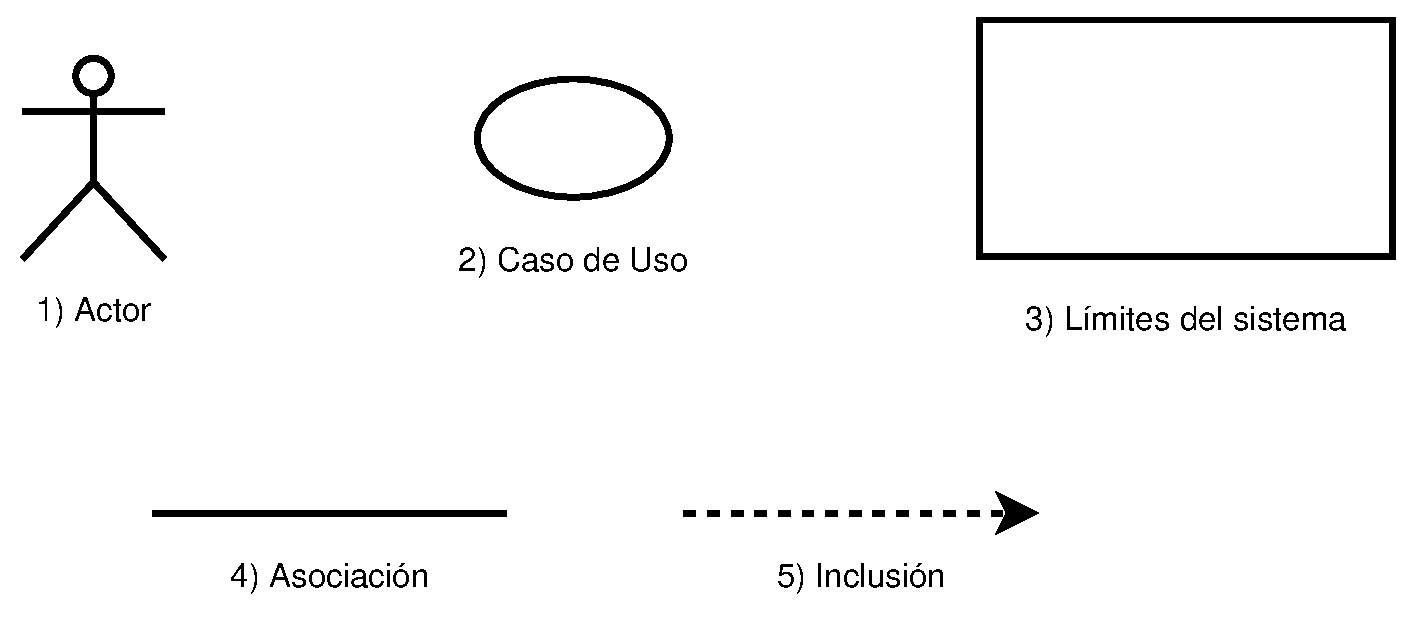
\includegraphics[scale=0.5]{uml-nota-use-case}
  \caption{Notación para diagramas de caso de uso\cite{SoftwareEngineeringUML}.}
  \label{fig:uml-nota-use-case}
\end{figure}

\section{Diagrama de actividad}\label{sec-uml-act}
Un diagrama de actividad modela el flujo de un proceso dentro del sistema, se compone de actividades y muestra las transiciones entre ellas, también puede ser utilizado para modelar la lógica de negocio\cite{UMLClassroom, SoftwareEngineeringUML}.\\
Un diagrama de actividad utiliza la siguiente notación\cite{UMLClassroom, SoftwareEngineeringUML} (ver Figura \ref{fig:uml-nota-activity}):
\begin{enumerate}
  \item \textbf{Inicio}: indica el inicio del flujo, se representa con un círculo.
  \item \textbf{Fin}: indica el fin del flujo, se presenta con un círculo dentro de una circunferencia, concéntricos.
  \item \textbf{Actividad}: es una acción dentro del diagrama, se representa con un rectángulo de esquinas redondeadas.
  \item \textbf{Flujo}: indica la secuencia entre actividades, se representa con una flecha.
  \item \textbf{Decisión}: es una bifurcación del flujo que depende de una condición, se representa con un rombo o diamante.
  \item \textbf{Conjunción}: es la unión entre flujos del diagrama, se representa con una barra rectangular.
  \item \textbf{Notas}: son observaciones a ciertos aspectos del diagrama\footnote{Este símbolo es utilizado en todos los diagramas UML}, se representa con un rectángulo que tiene un triángulo en la esquina superior derecha.
  \item \textbf{Partición}: indica la ejecución de actividades del sistema por parte de componentes del sistema o actores, se representa con con un rectángulo que contiene actividades y en el encabezado el identificador del componente o actor.
\end{enumerate}

\begin{figure}[h]
  \centering
  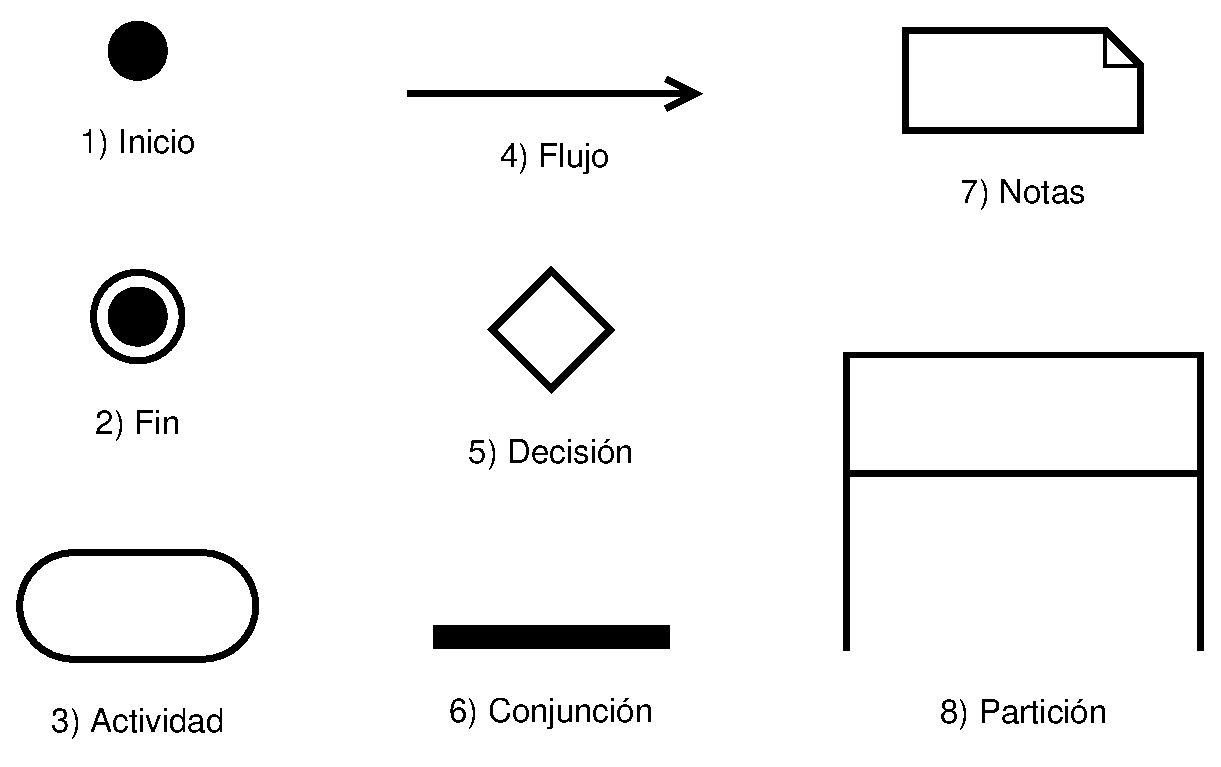
\includegraphics[scale=0.5]{uml-nota-activity}
  \caption{Notación para diagramas de actividad\cite{SoftwareEngineeringUML}.}
  \label{fig:uml-nota-activity}
\end{figure}

\section{Diagrama de componentes}\label{sec-uml-comp}
Un diagrama de componentes es la representación del sistema en unidades independientes del sistema\cite{UMLClassroom, SoftwareEngineeringUML}.\\
Un diagrama de actividad utiliza la siguiente notación\cite{UMLClassroom, SoftwareEngineeringUML} (ver Figura \ref{fig:uml-nota-component}):
\begin{enumerate}
  \item \textbf{Componente}: es una pieza independiente del sistema que provee servicios (interfaces) y consume servicios de otros componentes, se representa como un rectángulo con dos rectángulos más pequeños en columna superpuestos del lado izquierdo.
  \item \textbf{Interfaz}: es un conjunto de operaciones que ofrece el componente, se representa con un una circunferencia y una línea que une a la circunferencia con el componente.
  \item \textbf{Acoplamiento}: indica el consumo de una interfaz, se representa con media circunferencia que envuelve a una interfaz y se conecta al componente con una línea continua.
\end{enumerate}

\begin{figure}[h]
  \centering
  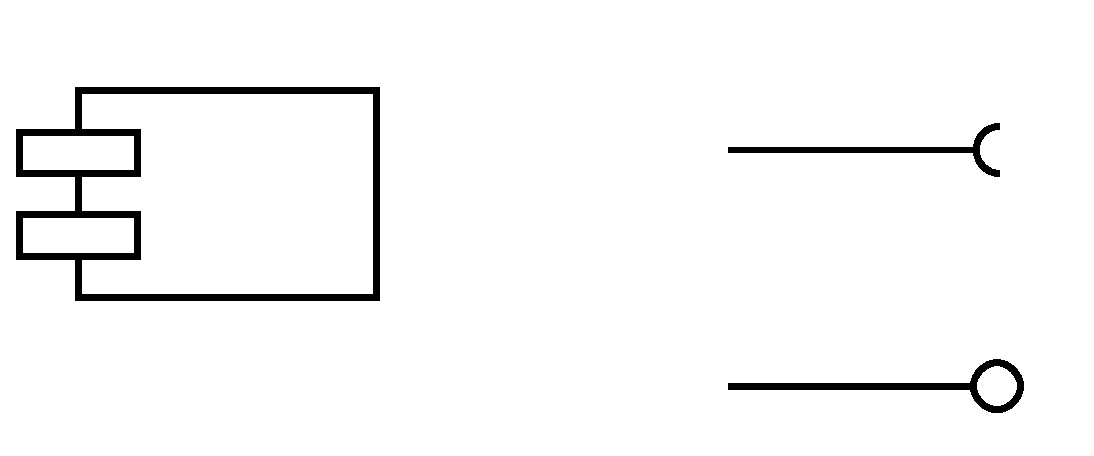
\includegraphics[scale=0.5]{uml-nota-component}
  \caption{Notación para diagramas de secuencia\cite{SoftwareEngineeringUML}.}
  \label{fig:uml-nota-component}
\end{figure}

\section{Diagrama de secuencia}\label{sec-uml-seq}
Un diagrama de secuencia describe las interacciones entre objetos para realizar una tarea, resalta la cronología de mensajes entre objetos así como la creación de estos\cite{UMLClassroom, SoftwareEngineeringUML}.\\
Un diagrama de secuencia utiliza la siguiente notación\cite{UMLClassroom, SoftwareEngineeringUML} (ver Figura \ref{fig:uml-nota-sequence}):
\begin{enumerate}
  \item \textbf{Actor}: ver descripción de \ref(sec-uml-cu).
  \item \textbf{Objeto}: es una parte del sistema que puede representar un rol, clase, componente o actor, se representa con un rectángulo con el nombre del objeto subrayado.
  \item \textbf{Mensaje}: es la comunicación entre dos objetos, se representa con una flecha de línea continua y tiene la descripción del mensaje.
  \item \textbf{Mensaje de retorno}: es un mensaje (en sentido contrario) que da respuesta a un mensaje anterior, se representa con una flecha de línea de guiones y tiene la descripción del contenido del mensaje.
  \item \textbf{Bloque}: es un conjunto de mensajes unidos bajo una estructura de control, se representa con un rectángulo que delimita una secuencia de mensajes y en la parte superior izquierda tiene la descripción del control de flujo dentro de un rectángulo.
  \item \textbf{Foco de control}: indica el tiempo que el objeto está activo durante el flujo, se representa como una barra vertical.
  \item \textbf{Línea de tiempo}: sirve como referencia de tiempo, es una línea punteada vertical que acompaña a un foco de control.
\end{enumerate}

\begin{figure}[h]
  \centering
  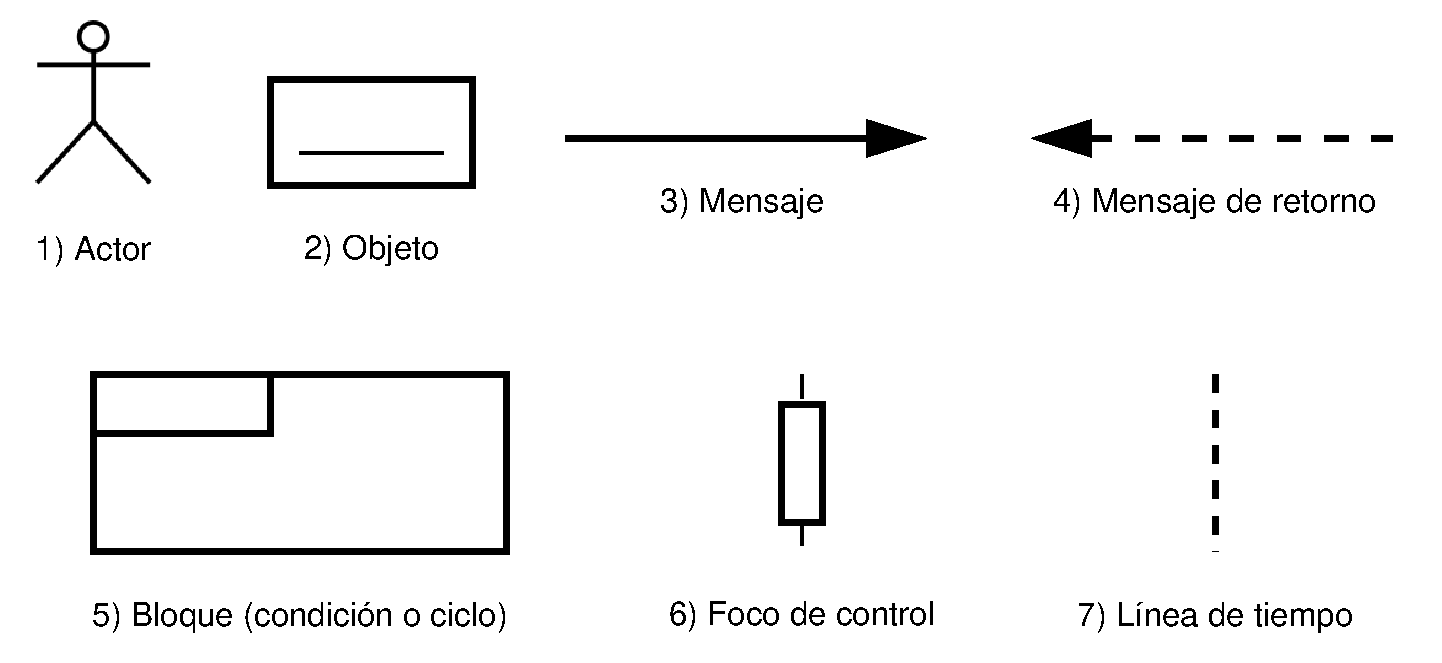
\includegraphics[scale=0.5]{uml-nota-sequence}
  \caption{Notación para diagramas de secuencia\cite{SoftwareEngineeringUML}.}
  \label{fig:uml-nota-sequence}
\end{figure}


%\section{Diagrama de clases}\label{sec-uml-class}
%\textcolor{blue}{lalalalalala}
